\section{Application à développer}

\subsection{Contexte}

Cette partie aborde le développement de l'application finale du projet, qui consiste à implanter un système de mesure du temps de réaction. L'objectif est d'évaluer la vitesse de réaction d'un utilisateur à un stimulus visuel géré par la carte SAMD21 et sa carte d'extension OLED1. Le système doit assurer un comportement fonctionnel et temporel rigoureux en s'appuyant sur les mécanismes de l'exécutif FreeRTOS, tels que les tâches, les sémaphores et les files de messages. \\

Le comportement séquentiel et temporel de la fonction centrale d'observation est régi par la machine à états présentée dans la figure ci-dessous. Elle gère les différentes phases du système : le repos, l'attente aléatoire d'un stimulus (allumage de la variable \textit{Sortie} sur les LED), la mesure du temps de réaction de l'utilisateur par comptage d'événements, ainsi que le calcul des statistiques (min, max, moyenne) transmises via une file de messages.

\begin{figure}[h]
    \centering
    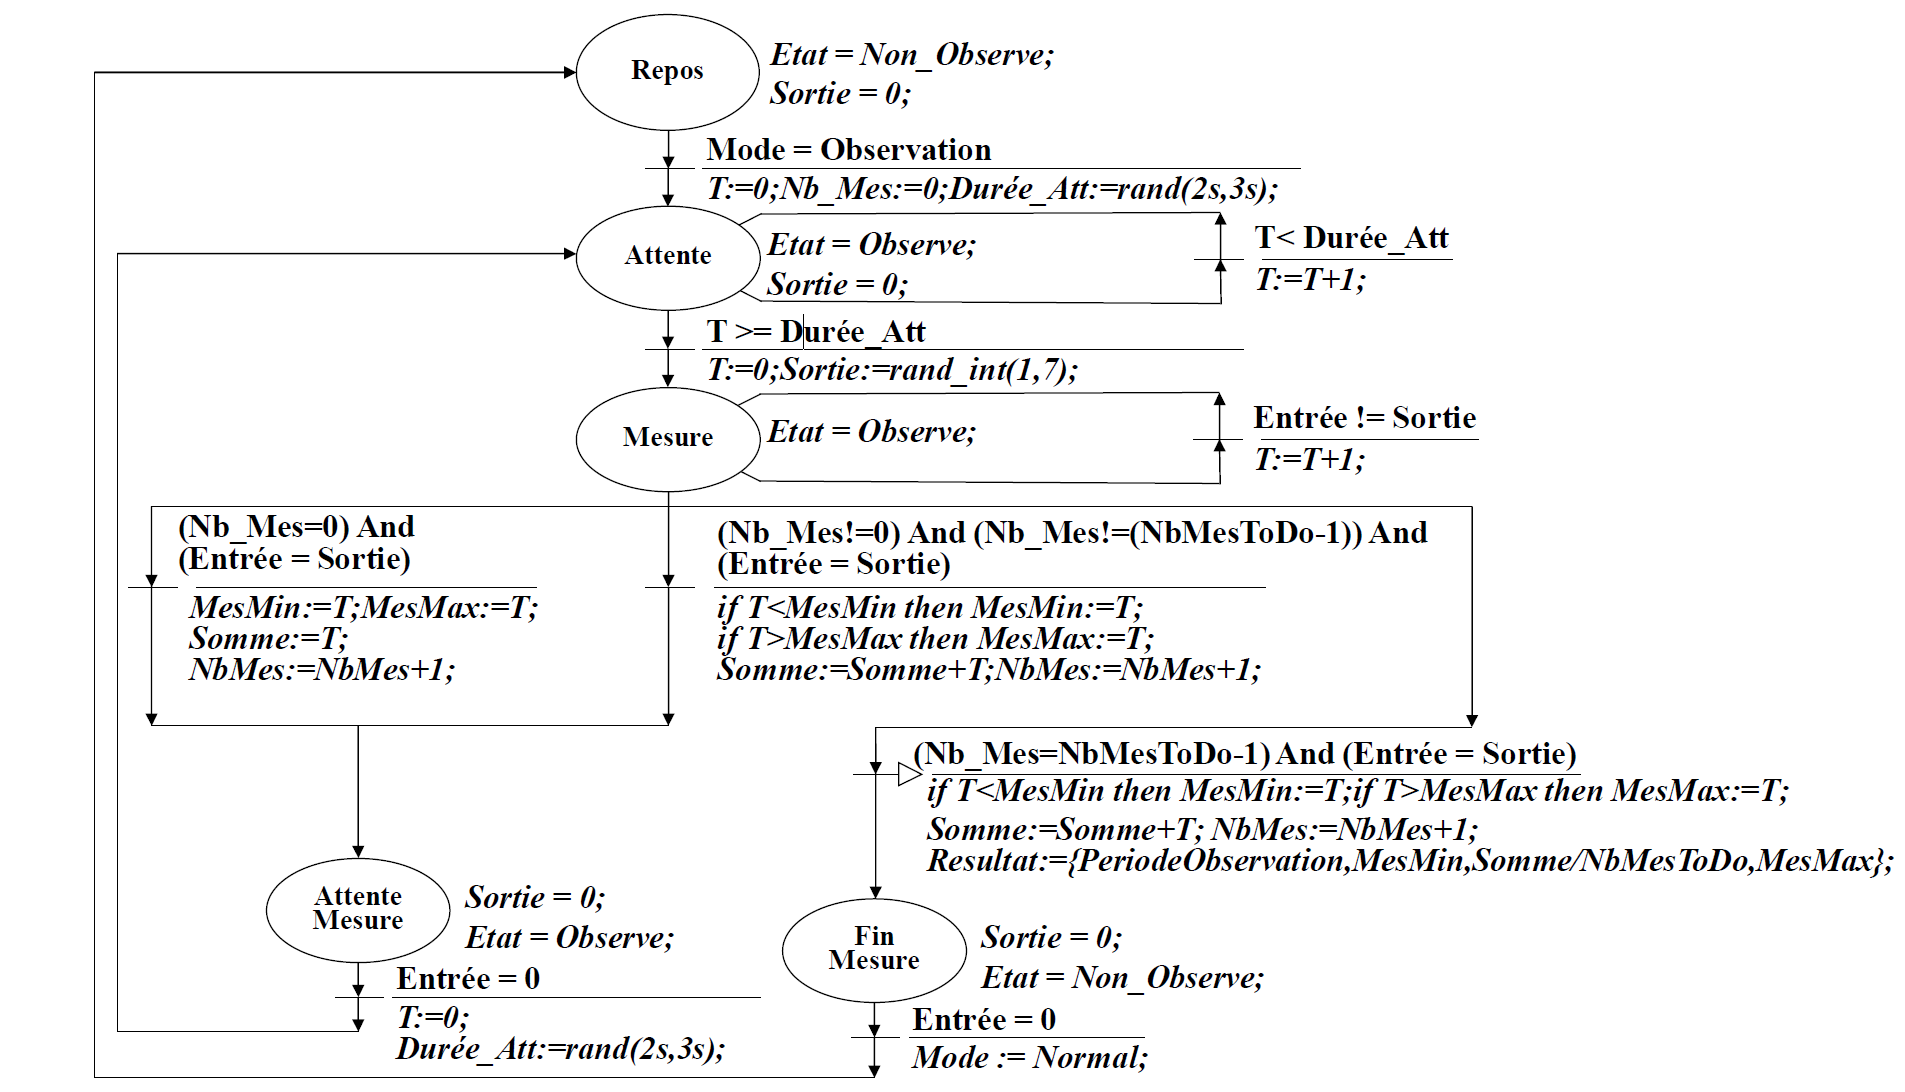
\includegraphics[width=0.8\linewidth]{Figures/fsm_observation.png}
    \caption{Comportement de la fonction Observation (machine à états)}
    \label{fig:machine_etats}
\end{figure}

\subsection{Analyse des besoins en éléments de RTOS pour l'application}

Pour concevoir cette application sous FreeRTOS, l'analyse fonctionnelle met en évidence plusieurs besoins structurants :
\begin{itemize}
    \item \textbf{Tâches (Tasks) :} L'application est découpée en quatre tâches distinctes hiérarchisées par leurs priorités :
    \begin{enumerate}
        \item \texttt{taskClock} (priorité haute) : Tâche périodique (cadencée à $1\text{ ms}$) servant d'horloge globale de référence.
        \item \texttt{taskSupervision} : Tâche chargée de scruter l'état du bouton de démarrage pour basculer en mode observation.
        \item \texttt{taskObservation} : Tâche centrale implémentant l'automate d'état, gérant les stimuli visuels et l'acquisition des boutons.
        \item \texttt{taskDisplay} : Tâche d'affichage passive restituant les statistiques sur l'écran OLED.
    \end{enumerate}
    \item \textbf{Sémaphores binaires :} \texttt{SemSupervision} et \texttt{SemObservation} synchronisent le réveil des tâches sur le tic d'horloge.
    \item \textbf{Mutex (Exclusion Mutuelle) :} \texttt{mutex\_mode} et \texttt{mutex\_oled1} protègent respectivement le mode et les accès concurrents au bus de la carte OLED1.
    \item \textbf{File de messages (Queue) :} \texttt{xQueueMeasurementResults} transfère le tableau des résultats statistiques vers l'affichage.
\end{itemize}

\subsection{Analyse et explication du code de l'application}

Le programme s'articule autour de l'initialisation matérielle (\texttt{system\_init}, \texttt{oled1\_init}, \texttt{ConfigureMeasure}), de la création des objets FreeRTOS, puis du lancement de l'ordonnanceur (\texttt{vTaskStartScheduler}). Le cœur du système repose sur la machine à états de la tâche d'observation (\texttt{REPOS}, \texttt{ATTENTE}, \texttt{MESURE}, \texttt{ATTENTE\_MESURE}, \texttt{FIN\_MESURE}) qui gère l'enchaînement des 5 mesures chronométrées. \\

\subsection{Preuves de fonctionnement de l'application}

Le bon comportement temporel de l'application a été validé sur la cible SAMD21 Xplained Pro avec la carte OLED1, garantissant une période d'observation stable voisine de $1\text{ ms}$. \\

Le résultat de cette exécution sur la carte SAMD21, confirmant le bon fonctionnement de l'application, est visible via ce lien : \href{https://youtube.com/shorts/WNDGfWiWxSI?feature=share}{\textbf{voir la démonstration vidéo sur YouTube}}. \\

\subsection{Code complet de l'application}

Le code source complet de l'application temps-réel FreeRTOS est présenté ci-dessous : \\

\begin{verbatim}
/* Inclusion des bibliothèques */
#include <asf.h>
#include <stdio.h>
#include <string.h>
#include <stdlib.h>
#include "FreeRTOS.h"
#include "task.h"
#include "semphr.h"
#include "timers.h"

#include "oled1.h"
#include "MesTemps.h"
#include "gfx_mono.h"
#include "gfx_mono_text.h"
#include "sysfont.h"

#define OLED1_EXT_HEADER      EXT1
static OLED1_CREATE_INSTANCE(oled1, OLED1_EXT_HEADER);

#define TASK_CLOCK_PRIORITY        (tskIDLE_PRIORITY + 4)
#define TASK_SUPERVISION_PRIORITY  (tskIDLE_PRIORITY + 3)
#define TASK_OBSERVATION_PRIORITY  (tskIDLE_PRIORITY + 2)
#define TASK_DISPLAY_PRIORITY      (tskIDLE_PRIORITY + 1)

#define HORLOGE_TASK_DELAY         1
#define NBMES_TO_DO                5

static SemaphoreHandle_t SemSupervision = NULL;
static SemaphoreHandle_t SemObservation = NULL;
static SemaphoreHandle_t mutex_mode     = NULL;
static SemaphoreHandle_t mutex_oled1    = NULL;
static QueueHandle_t xQueueMeasurementResults = NULL; 

void vSetupHardware(void);
void taskClock(void *pvParameters);
void taskSupervision(void *pvParameters);
void taskObservation(void *pvParameters);
void taskDisplay(void *pvParameters);

typedef enum {
    REPOS,
    ATTENTE,
    MESURE,
    ATTENTE_MESURE,
    FIN_MESURE
} StateForObservation;

typedef enum {
    Normal,
    Observation
} Mode;

static Mode mode = Normal;
static uint16_t measurementResults[4];

static uint16_t T = 0;
static uint16_t Nb_Mes = 0;
static uint16_t Duree_Att = 0;
static uint16_t MesMin = 0;
static uint16_t MesMax = 0;
static uint32_t Somme = 0;
static uint8_t  Sortie_val = 0;

uint8_t get_entree_buttons(void)
{
    uint8_t val = 0;
    if (xSemaphoreTake(mutex_oled1, portMAX_DELAY) == pdTRUE) {
        if (oled1_get_button_state(&oled1, OLED1_BUTTON1_ID)) val |= 0x01;
        if (oled1_get_button_state(&oled1, OLED1_BUTTON2_ID)) val |= 0x02;
        if (oled1_get_button_state(&oled1, OLED1_BUTTON3_ID)) val |= 0x04;
        xSemaphoreGive(mutex_oled1);
    }
    return val;
}

void set_sortie_leds(uint8_t val)
{
    if (xSemaphoreTake(mutex_oled1, portMAX_DELAY) == pdTRUE) {
        oled1_set_led_state(&oled1, OLED1_LED1_ID, (val & 0x01) ? true : false);
        oled1_set_led_state(&oled1, OLED1_LED2_ID, (val & 0x02) ? true : false);
        oled1_set_led_state(&oled1, OLED1_LED3_ID, (val & 0x04) ? true : false);
        xSemaphoreGive(mutex_oled1);
    }
}

void set_etat_led0(bool observe)
{
    if (observe) {
        port_pin_set_output_level(LED_0_PIN, LED_0_ACTIVE);
    } else {
        port_pin_set_output_level(LED_0_PIN, !LED_0_ACTIVE);
    }
}

void vSetupHardware(void)
{
    system_init();       
    gfx_mono_init();     
    oled1_init(&oled1);  
    ConfigureMeasure();  
}

int main(void)
{
    vSetupHardware();

    gfx_mono_draw_filled_rect(0, 0, GFX_MONO_LCD_WIDTH, GFX_MONO_LCD_HEIGHT, GFX_PIXEL_CLR);
    gfx_mono_draw_string("READY - Press SW0", 0, 0, &sysfont);

    srand(1234); 

    SemSupervision = xSemaphoreCreateBinary();
    SemObservation = xSemaphoreCreateBinary();
    mutex_mode     = xSemaphoreCreateMutex();
    mutex_oled1    = xSemaphoreCreateMutex();
    xQueueMeasurementResults = xQueueCreate(1, sizeof(measurementResults));

    xTaskCreate(taskClock,       "Clock",       configMINIMAL_STACK_SIZE,     NULL, TASK_CLOCK_PRIORITY,       NULL);
    xTaskCreate(taskSupervision, "Supervision", configMINIMAL_STACK_SIZE,     NULL, TASK_SUPERVISION_PRIORITY, NULL);
    xTaskCreate(taskObservation, "Observation", configMINIMAL_STACK_SIZE * 2, NULL, TASK_OBSERVATION_PRIORITY, NULL);
    xTaskCreate(taskDisplay,     "Display",     configMINIMAL_STACK_SIZE * 3, NULL, TASK_DISPLAY_PRIORITY,     NULL);

    StartMeasure();
    vTaskStartScheduler();

    for (;;);
}

void taskClock(void *pvParameters)
{
    (void) pvParameters;
    for (;;)
    {
        vTaskDelay(pdMS_TO_TICKS(HORLOGE_TASK_DELAY));
        xSemaphoreGive(SemSupervision);
        xSemaphoreGive(SemObservation);
    }
}

void taskSupervision(void *pvParameters)
{
    (void) pvParameters;
    bool Start;
    bool StartPrec = false;

    for (;;)
    {
        xSemaphoreTake(SemSupervision, portMAX_DELAY);
        Start = (port_pin_get_input_level(BUTTON_0_PIN) == BUTTON_0_ACTIVE);

        if ((StartPrec == false) && (Start == true))
        {
            if (xSemaphoreTake(mutex_mode, portMAX_DELAY) == pdTRUE)
            {
                if (mode == Normal) mode = Observation;
                xSemaphoreGive(mutex_mode);
            }
        }
        StartPrec = Start;
    }
}

void taskObservation(void *pvParameters)
{
    (void) pvParameters;
    StateForObservation PresState = REPOS;
    StateForObservation NextState = REPOS;
    uint16_t periodeObservation_us = 0;

    for (;;)
    {
        xSemaphoreTake(SemObservation, portMAX_DELAY);
        periodeObservation_us = EndMeasure();
        StartMeasure();

        PresState = NextState;

        Mode current_mode = Normal;
        if (xSemaphoreTake(mutex_mode, portMAX_DELAY) == pdTRUE) {
            current_mode = mode;
            xSemaphoreGive(mutex_mode);
        }

        switch (PresState)
        {
            case REPOS:
                set_etat_led0(false);
                set_sortie_leds(0);
                if (current_mode == Observation)
                {
                    T = 0;
                    Nb_Mes = 0;
                    Duree_Att = 2000 + (rand() % 1001);
                    NextState = ATTENTE;
                }
                break;

            case ATTENTE:
                set_etat_led0(true);
                set_sortie_leds(0);
                if (T < Duree_Att)
                {
                    T = T + 1;
                    NextState = ATTENTE;
                }
                else
                {
                    T = 0;
                    Sortie_val = 1 + (rand() % 7);
                    set_sortie_leds(Sortie_val);
                    NextState = MESURE;
                }
                break;

            case MESURE:
            {
                set_etat_led0(true);
                uint8_t entree = get_entree_buttons();

                if (entree != Sortie_val)
                {
                    T = T + 1;
                    NextState = MESURE;
                }
                else
                {
                    if (Nb_Mes == 0)
                    {
                        MesMin = T; MesMax = T; Somme = T;
                        Nb_Mes++; set_sortie_leds(0);
                        NextState = ATTENTE_MESURE;
                    }
                    else if (Nb_Mes < (NBMES_TO_DO - 1))
                    {
                        if (T < MesMin) MesMin = T;
                        if (T > MesMax) MesMax = T;
                        Somme += T; Nb_Mes++; set_sortie_leds(0);
                        NextState = ATTENTE_MESURE;
                    }
                    else
                    {
                        if (T < MesMin) MesMin = T;
                        if (T > MesMax) MesMax = T;
                        Somme += T; Nb_Mes++;

                        measurementResults[0] = periodeObservation_us;
                        measurementResults[1] = MesMin;
                        measurementResults[2] = (uint16_t)(Somme / NBMES_TO_DO);
                        measurementResults[3] = MesMax;

                        xQueueSend(xQueueMeasurementResults, &measurementResults, 0);
                        set_sortie_leds(0);
                        set_etat_led0(false);
                        NextState = FIN_MESURE;
                    }
                }
                break;
            }

            case ATTENTE_MESURE:
                set_sortie_leds(0);
                set_etat_led0(true);
                if (get_entree_buttons() == 0)
                {
                    T = 0;
                    Duree_Att = 2000 + (rand() % 1001);
                    NextState = ATTENTE;
                }
                break;

            case FIN_MESURE:
                set_sortie_leds(0);
                set_etat_led0(false);
                if (get_entree_buttons() == 0)
                {
                    if (xSemaphoreTake(mutex_mode, portMAX_DELAY) == pdTRUE) {
                        mode = Normal;
                        xSemaphoreGive(mutex_mode);
                    }
                    NextState = REPOS;
                }
                break;
        }
    }
}

void taskDisplay(void *pvParameters)
{
    (void) pvParameters;
    char buf[24];
    uint16_t receivedResults[4];

    for (;;)
    {
        if (xQueueReceive(xQueueMeasurementResults, &receivedResults, portMAX_DELAY) == pdTRUE)
        {
            if (xSemaphoreTake(mutex_oled1, portMAX_DELAY) == pdTRUE)
            {
                gfx_mono_draw_filled_rect(0, 0, GFX_MONO_LCD_WIDTH, GFX_MONO_LCD_HEIGHT, GFX_PIXEL_CLR);

                snprintf(buf, sizeof(buf), "Per: %u us", receivedResults[0]);
                gfx_mono_draw_string(buf, 0, 0, &sysfont);

                snprintf(buf, sizeof(buf), "Min: %u ms", receivedResults[1]);
                gfx_mono_draw_string(buf, 0, 8, &sysfont);

                snprintf(buf, sizeof(buf), "Moy: %u ms", receivedResults[2]);
                gfx_mono_draw_string(buf, 0, 16, &sysfont);

                snprintf(buf, sizeof(buf), "Max: %u ms", receivedResults[3]);
                gfx_mono_draw_string(buf, 0, 24, &sysfont);

                xSemaphoreGive(mutex_oled1);
            }
        }
    }
}
\end{verbatim}